\documentclass[12pt, twoside]{article}
\documentclass[12pt, twoside]{article}
\usepackage[letterpaper, margin=1in, headsep=0.2in]{geometry}
\setlength{\headheight}{0.6in}
%\usepackage[english]{babel}
\usepackage[utf8]{inputenc}
\usepackage{microtype}
\usepackage{amsmath}
\usepackage{amssymb}
%\usepackage{amsfonts}
\usepackage{siunitx} %units in math. eg 20\milli\meter
\usepackage{yhmath} % for arcs, overparenth command
\usepackage{tikz} %graphics
\usetikzlibrary{quotes, angles}
\usepackage{graphicx} %consider setting \graphicspath{{images/}}
\usepackage{parskip} %no paragraph indent
\usepackage{enumitem}
\usepackage{multicol}
\usepackage{venndiagram}

\usepackage{fancyhdr}
\pagestyle{fancy}
\fancyhf{}
\renewcommand{\headrulewidth}{0pt} % disable the underline of the header
\raggedbottom
\hfuzz=2mm %suppresses overfull box warnings

\usepackage{hyperref}
\usepackage{float}

\title{Algebra 2}
\author{Chris Huson}
\date{May 2024}

\fancyhead[LE]{\thepage}
\fancyhead[RO]{\thepage \\ Name: \hspace{1.5cm} \,\\}
\fancyhead[LO]{BECA/Huson/Algebra 2: Regents Preparation \\* 23 May 2024}

\begin{document}

\subsubsection*{Prep \#16 Polynomials and algebra}
\begin{enumerate}[itemsep=0.5cm]

\item Simplify each expression.
    \begin{multicols}{2}
    \begin{enumerate}[itemsep=0.75cm]
        \item $\displaystyle x^{\frac{2}{3}} \cdot x^{\frac{1}{3}} =$
        \item $\displaystyle x^{\frac{4}{5}} \cdot x^{\frac{6}{5}} =$
        \item $\displaystyle \frac{\sqrt[3]{8x^2}}{\sqrt{16x}} = $
        \item $\displaystyle (x^{\frac{3}{2}}y^3)^2 =$
        \item $\displaystyle (x^{\frac{2}{3}}y^4)^{\frac{1}{2}} =$
        \item $\displaystyle \frac{x^{\frac{3}{4}}}{x^{\frac{1}{4}}} =$
    \end{enumerate}
    \end{multicols} \vspace{0.5cm}

\item Write the expression as a polynomial in standard form.
    \begin{multicols}{2}
    \begin{enumerate}
        \item $(x-3)(x+3)$
        \item $(x+y)(x^2-xy+y^2)$
    \end{enumerate}
    \end{multicols} \vspace{3cm}

\item Simplify each complex expression to the form $a+bi$, with real numbers $a$ and $b$.
    \begin{multicols}{2}
    \begin{enumerate}[itemsep=4cm]
        \item $(2+3i)(3-4i)=$
        \item $(2xi+4)^2=$
        \item $(2xi+4)^2=$
        \item $-2i(\sqrt{-3}+4i)-5i^3$
    \end{enumerate}
    \end{multicols} \vspace{3cm}

\newpage
The quadratic formula:
$\displaystyle x = \frac{-b \pm \sqrt{b^2-4ac}}{2a}$

\item Solve each equation. Expression the answer in $a+bi$ form.
    \begin{multicols}{2}
    \begin{enumerate}[itemsep=0.5cm]
        \item $2x^2+5x+8=0$
        \item $3x^2+7x+5=0$
    \end{enumerate}
    \end{multicols} \vspace{5cm}

\item Determine the solution of each equation algebraically.
    \begin{multicols}{2}
    \begin{enumerate}[itemsep=0.5cm]
        \item $\sqrt{3x+7}=x-1$ %June 2023
        \item $\sqrt{4x+1} = 11-x$ %Aug 2022
        %\item $\sqrt{49-10x} + 5 = 2x$ %Jan 2023
        %\item $\sqrt{6-2x} + x = 2(x+15)-9$ %June 2018
        %\item $2x = 6+2\sqrt{x-1}$ %Jan 2024
        %\item $3\sqrt{x} -2x = -5$ %Jan 2019
    \end{enumerate}
    \end{multicols}

\newpage
Geometric Series:
$$S_n = \frac{a_1 - a_1 r^n}{1-r} \text{ where } r \ne 1$$

\item Write a recursive formula for the sequence 16, 8, 0, $-8$, $\ldots$ \vspace{2cm}

\item A sequence is defined by the recursive formula
\begin{align*}
a_1 &= 30 \\
a_{n} &= a_{n-1}+5
\end{align*}
Write an explicit formula for the sequence. \vspace{2cm}


\item The sum of the first $n$ terms of the geometric sequence beginning $1$, $1.5$, $2.25$, $\ldots$ is 171, rounded to \emph{the nearest integer}. Find $n$. \vspace{2cm}

%F.LE.2: Construct a linear or exponential function symbolically given: a graph, a description of the relationship, or two input-output pairs (including from a table).
\item Complete the table for the geometric sequence $a$.
    \begin{center}
    \begin{tabular}{|p{1cm}|p{1cm}|p{1cm}|p{1cm}|p{1cm}|p{1cm}|}
        \hline
        $n$ & 1 & 2 & 3 & 4 & 5 \\
        \hline
        $a_n$ & 100 & 80 & & & \\[0.25cm]
        \hline
    \end{tabular}
    \end{center}
    Model the sequence with an exponential function.


\newpage
\item A survey was conducted to compare the dietary habits of American and Japanese families. Families were asked which they had eaten for dinner most recently, meat or fish. The proportions of each answer are shown in the table below.
    \begin{center}
        \begin{tabular}{|c|c|c|c|}
            \hline
            Nationality & Meat & Fish & Total \\[0.2cm]
            \hline
            Americans & 0.78 & 0.22 & 1.00 \\[0.25cm]
            \hline
            Japanese & 0.43 & 0.57 & 1.00 \\[0.25cm]
            \hline
        \end{tabular}
    \end{center}
    \begin{enumerate}
        \item Does the survey data indicate that Americans and Japanese families have similiar dietary habits? Justify your answer. \vspace{2cm}
        \item 200 American families and 100 Japanese families participated in the survey. Calculate the number of each category of response and enter it in the appropriate cell in the table below. 
        \begin{center}
            \begin{tabular}{|c|p{1.5cm}|p{1.5cm}|c|}
                \hline
                Nationality & \; Meat & \; Fish & Total \\[0.2cm]
                \hline
                Americans & &  & 200 \\[0.25cm]
                \hline
                Japanese & &  & 100 \\[0.25cm]
                \hline
            \end{tabular}
        \end{center}
        \item The survey was conducted in Kansas City (an inland city) and Tokyo (a city on the Pacific Ocean). How might that affect the survey's findings? 
    \end{enumerate} \vspace{3cm}

    \begin{multicols}{2}
\item An exponential function $f(x)$ is graphed.
\begin{enumerate}
    \item Write down an equation for $f(x)$.\vspace{1.5cm}
    \item Find the average rate of change of the function over the interval $0 < x < 4$.
    \vspace{2cm}
\end{enumerate}
    \begin{flushright}
        \begin{tikzpicture}[x=1cm, y=0.1cm, xscale=1.5]
            \draw [thin, color=lightgray, xstep=1cm,ystep=0.5cm] (0,0) grid (4,51);
            \draw [thick, ->] (0,0) -- (+4.3,0) node [below]{$x$};
            \draw [thick, ->] (0,0) -- (0,53) node [right]{$y$};        
            \foreach \x in {0,1,...,4}
                \draw (\x cm,5pt) -- (\x cm,-5pt) node[below] {$\x$};
            \foreach \y in {0,10,...,50}
                \draw[shift={(0,\y)}] (2pt,0pt)--(-2pt,0pt) node[left]{$\y$};
            \draw [thick, ->, smooth,domain=0.:4.2] plot(\x,{15*(3^(\x/4))});
            \fill (0,15) ellipse [x radius=1.33pt, y radius=2pt];
            \fill (4,45) ellipse [x radius=1.33pt, y radius=2pt];
        \end{tikzpicture}
        \end{flushright}
    \end{multicols}
\newpage
AII-F.LE.2: Construct a linear or exponential function symbolically given: a graph, a description of the relationship, or two input-output pairs (include reading these from a table).

\item Given the cubic function $f(x) = -x^3+4x^2+x-4$, graphed below.
\begin{enumerate}[itemsep=1cm]
    \item How many real solutions are their to the equation $f(x)=0$?
    \item Write down the real zeros of the function.
    \item Over the interval $3 < x < 4$, is the function increasing, decreasing, or constant?
    \item Find the average rate of change of the function over the interval from point $A$ to point $B$. \vspace{2cm}
\end{enumerate}
\begin{center}
    \begin{tikzpicture}[scale=0.5]
        \draw[gray,thin] (-10,-9) grid (10,9);
        \draw [thick,<->] (-10.5,0)--(10.5,0) node [right] {$x$};
        \draw [thick,<->] (0,-9.5)--(0,9.5) node [above] {$f(x)$};
        \draw [thick,<->] plot[smooth, domain=-1.6:4.3] (\x, {-(\x*\x-1)*(\x-4)});
        \fill (1,0) circle[radius=0.15] node [below right] {$A(1,0)$};
        \fill (3,8) circle[radius=0.15] node [right] {$B(3,8)$};
    \end{tikzpicture}
    \end{center}

\newpage
\item Factor the function $f(x) = x^3+4x^2-4x-16$ over the set of integers. \vspace{10cm}

\item Given the function $f(x) = x^3-2x^2-9x+18$, find the value of $f(2)$.\\[5cm]
Now identify the correct statement.
\begin{enumerate}
    \item $f(2)=0$ and $x-2$ is a factor of $f(x)$.
    \item $f(2)=0$ and $x-2$ is not a factor of $f(x)$.
    \item $f(2) \ne 0$ and $x-2$ is a factor of $f(x)$.
    \item $f(2) \ne 0$ and $x-2$ is not a factor of $f(x)$.
\end{enumerate}

\newpage
\item Graph the continuous exponential function $f(x) = 3e^{0.10x}$ on the grid below. 
\begin{center}
    \begin{tikzpicture}[scale=1]
        \draw[gray,thin] (0,0) grid (10,10);
        \draw [thick,->] (0,0)--(10.5,0) node [right] {$x$};
        \draw [thick,->] (0,0)--(0,10.5) node [above] {$f(x)$};
        \foreach \x in {0,1,...,10}
            \draw (\x cm,5pt) -- (\x cm,-5pt) node[below] {$\x$};
        \foreach \y in {0,1,...,10}
            \draw[shift={(0,\y)}] (2pt,0pt)--(-2pt,0pt) node[left]{$\y$};
    \end{tikzpicture}
    \end{center}
    \begin{enumerate}
        \item Graph the line $y=6$. Mark the intersection of the line with $f$ and label it as an ordered pair, rounded \emph{the nearest whole number}.
        \item The function $f(x)$ models the growth of an investment. Explain what the values of $3$ and $0.10$ represent in the context of the investment. \vspace{4cm}
        \item How long will the investment take to double? 
    \end{enumerate}

\end{enumerate}
\end{document}

3.OA.7
Fluently multiply and divide within 100, using such as the relationship between multiplication and division. By the end of Grade 3, know from memory all products of two one-digit numbers.
